\cfoot{Samuel Schober}
Der "`Homeponic-Prototyp"' ist ein Aufsatz für Aquarien und wurde von dem Projekt Partner Ponix Systems designed und zur Verfügung gestellt. In der Evaluierung (Kapitel 4) wird beschrieben, warum der Prototyp von Ponix Systems bezogen wurde. Da der Aquariumaufsatz bei Ponix Systems hauptsächlich für Testzwecke verwendet wurde, mussten für die Ausführung im Umfang des Diplomprojekts Modifizierungen getätigt werden. Die folgenden Überschriften beschreiben den anfänglichen Aufbau und welche Modifizierungen getätigt wurden, sodass die Bedürfnisse des Teams gedeckt waren.\\
\mbox{} \\
\mbox{} \\
\mbox{} \\
\mbox{} \\
\newpage
\subsubsection{Grundaufbau}
Der Prototyp Aufsatz bestand aus den folgenden Einzelteilen:
\begin{itemize}
    \item{Aquariumaufsatz}\mbox{} \\
    \begin{figure}[ht]
        \centering
        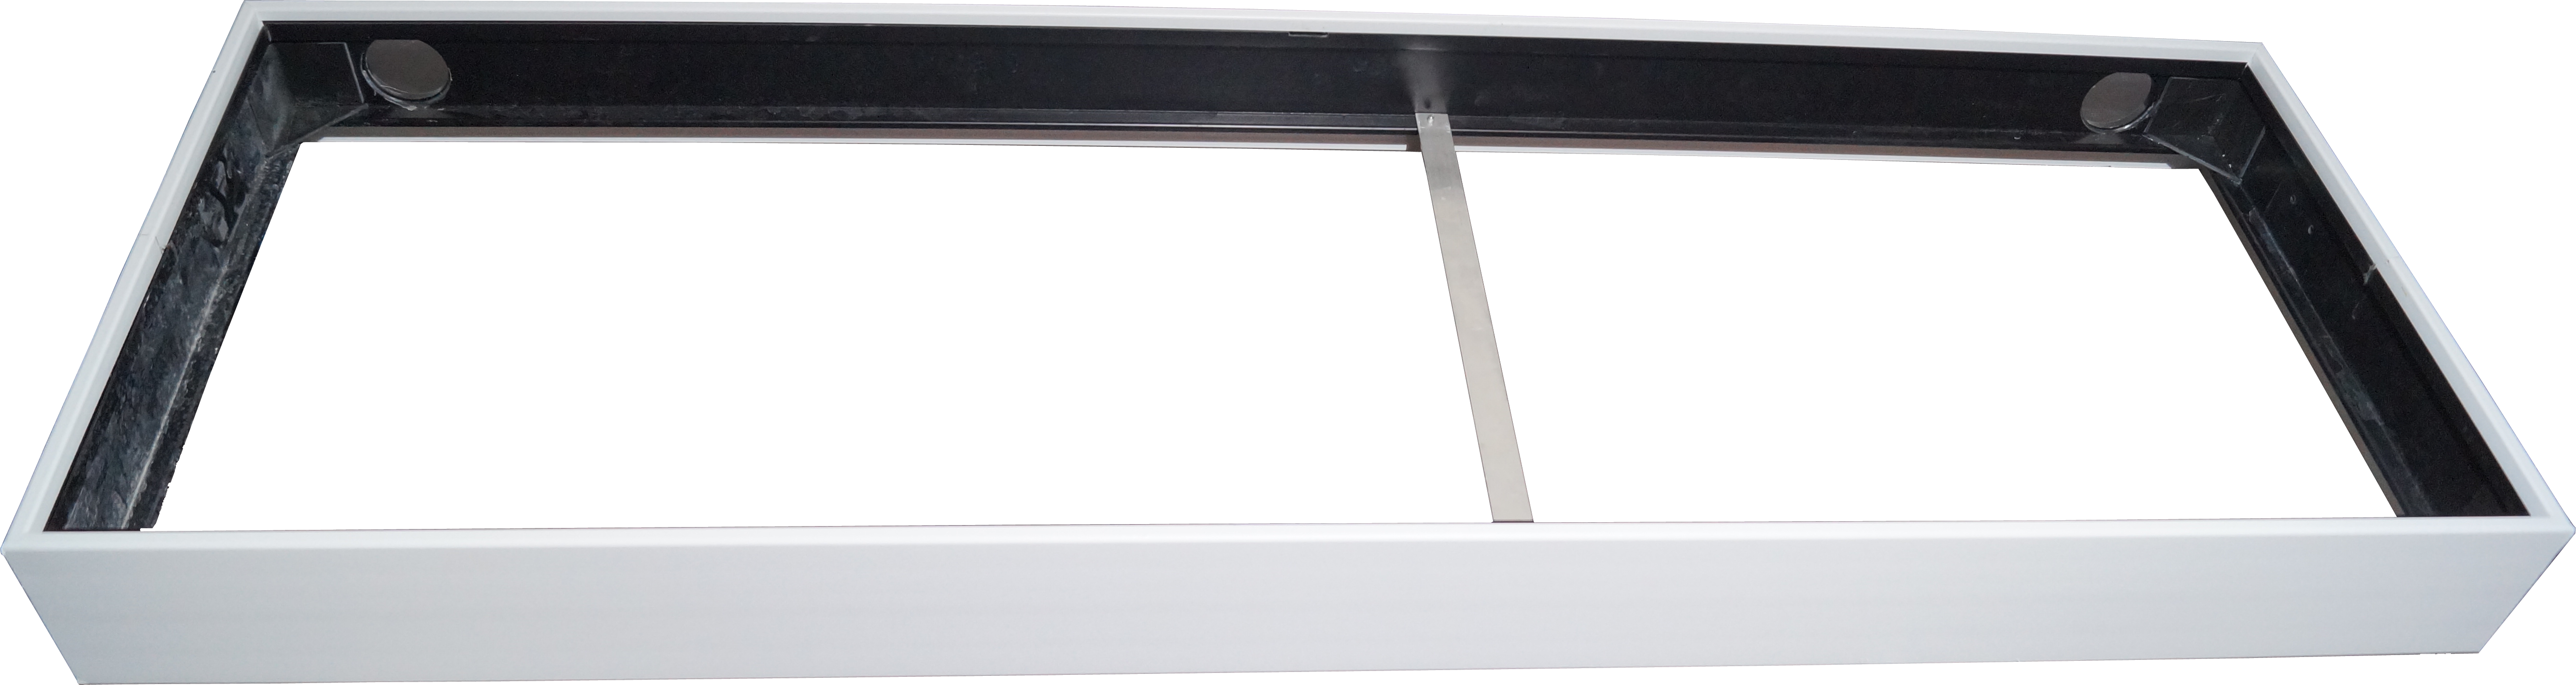
\includegraphics[width=0.5\textwidth]{images/Aufsatz}
	    \caption{Aquariumaufsatz}
    \end{figure}
    \item{Abdeckungen des Aquariumaufsatzes}\mbox{} \\
    \begin{figure}[ht]
        \centering
        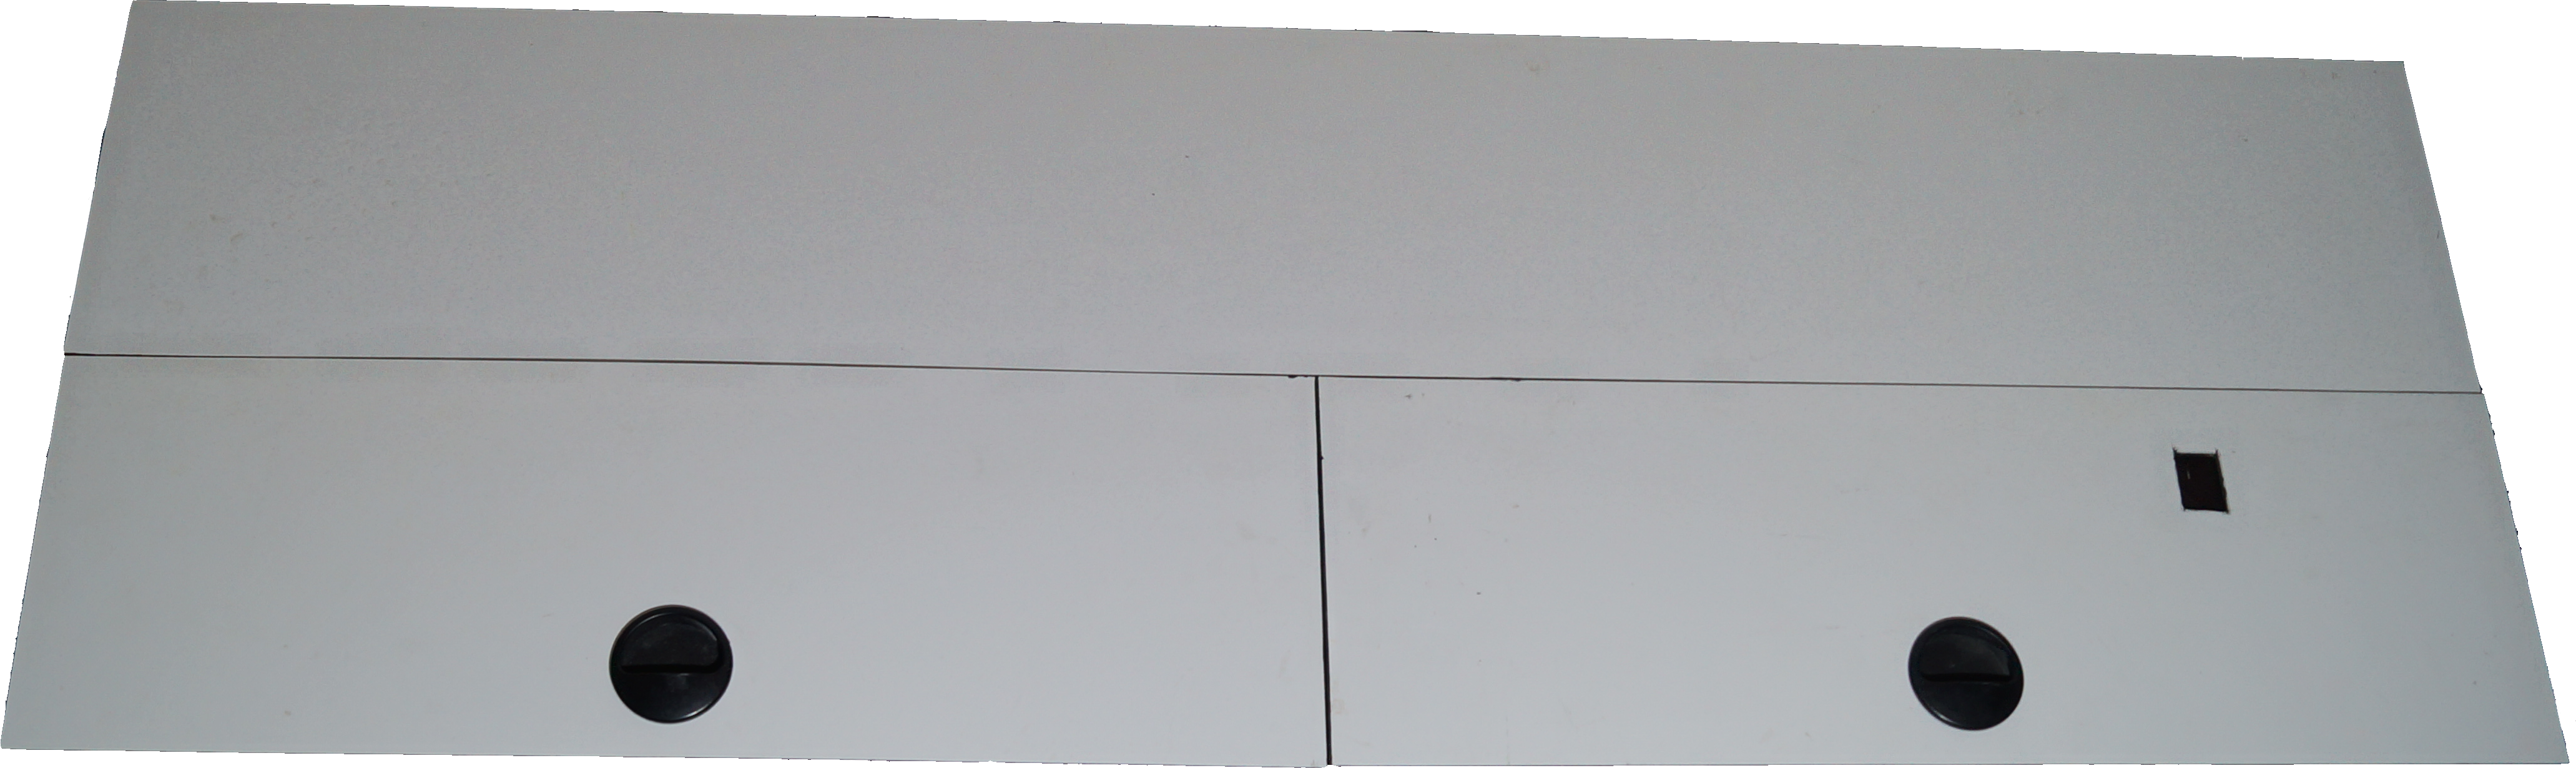
\includegraphics[width=0.5\textwidth]{images/Abdeckungen}
	    \caption{Abdeckungen des Aquariumaufsatzes}
    \end{figure}
    \item{\gls{NFT}-Kanal}\mbox{} \\
    \begin{figure}[ht]
        \centering
        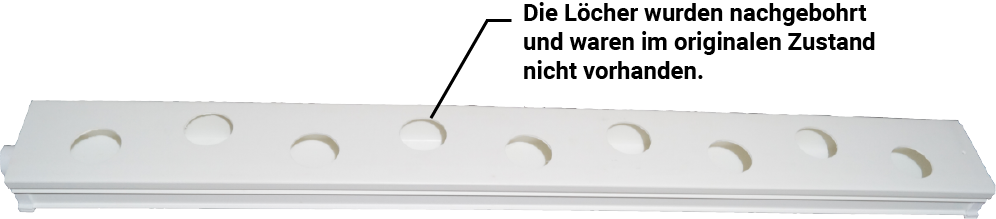
\includegraphics[width=0.5\textwidth]{images/NFT-Kanal}
	    \caption{\gls{NFT}-Kanal}
    \end{figure}
    \newpage
    \item{LED-Bretter}\mbox{} \\
    \begin{figure}[ht]
       \centering
       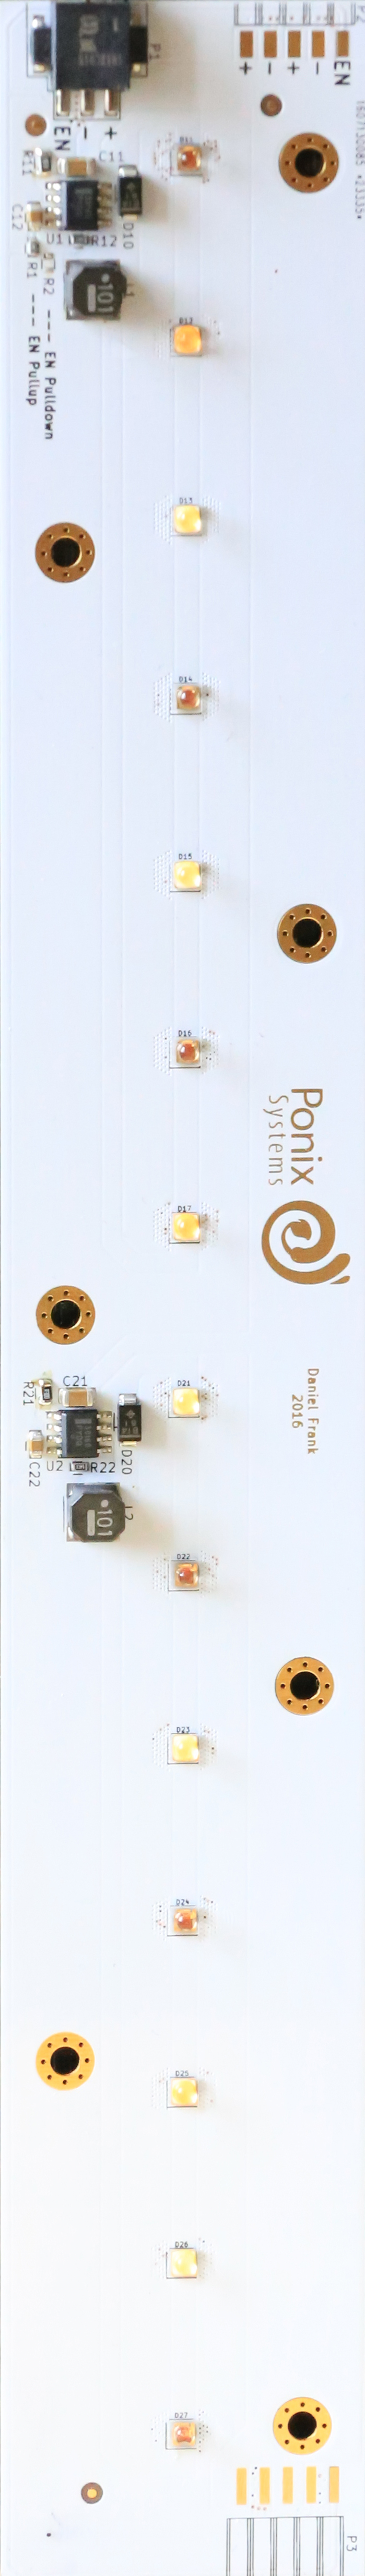
\includegraphics[height=0.5\textwidth, angle=90]{images/pflanzenLicht}
	   \caption{LED-Brett}
    \end{figure}
    \item{Halterung der \gls{LED}-Bretter}\mbox{} \\
    \begin{figure}[ht]
        \centering
        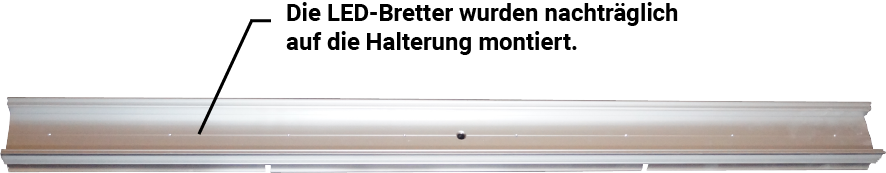
\includegraphics[width=0.5\textwidth]{images/LED-Halterung}
	    \caption{Halterung der LED-Bretter}
    \end{figure}
\end{itemize}

Die Fertigstellung des "`Homeponic-Prototypen"' mit diesen Teilen benötigte noch weiterer Modifizierungen des Aquariumaufsatzes, sowie die Beschaffung und Bearbeitung der nicht zur Verfügung gestellten Teile.\mbox{} \\
\mbox{} \\
\mbox{} \\
\mbox{} \\
\newpage
\subsubsection{Modifizierungen}
In den folgenden Schritten werden die Prozesse definiert, welche stattfanden, um den "`Homeponic-Prototypen"' einsatzbereit zu machen. Die Wahl des Werkstoffes fiel bei den Modifizierungen immer auf Aluminium, weil dieses im Gegensatz zu einigen anderen Metallen den Vorteil hat, leicht und gut bearbeitbar zu sein, außerdem rostet es kaum bis gar nicht.\\

\begin{description}
    \item [Querbalken für die Abdeckungen]\mbox{} \\
    Um die Aquarium Abdeckungen stabiler zu machen wurde ein Querbalken in den Aufsatz eingebaut. Dieser Querbalken ist ein Aluminium T-Profil mit einer Länge von 129 cm.
    \begin{figure}[ht]
        \centering
        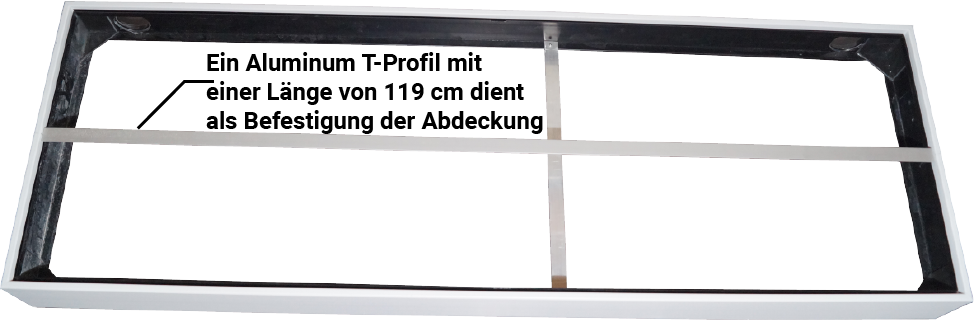
\includegraphics[width=0.5\textwidth]{images/Aufsatz_Mod}
	    \caption{Aquariumaufsatz mit eingebautem Querbalken}
    \end{figure}
    \item [Halterungsschienen des \gls{NFT}-Kanals]\mbox{} \\
    Für den \gls{NFT}-Kanal wurden noch Befestigungen benötigt, sodass er in den Aquariumaufsatz eingebaut werden kann. Hierfür wurden zwei Aluminium L-Profile (eines für jedes Ende des \gls{NFT}-Kanals) auf eine Länge von 38,2 cm zurechtgeschnitten und in den Aufsatz eingesetzt.
    \begin{figure}[ht]
        \centering
        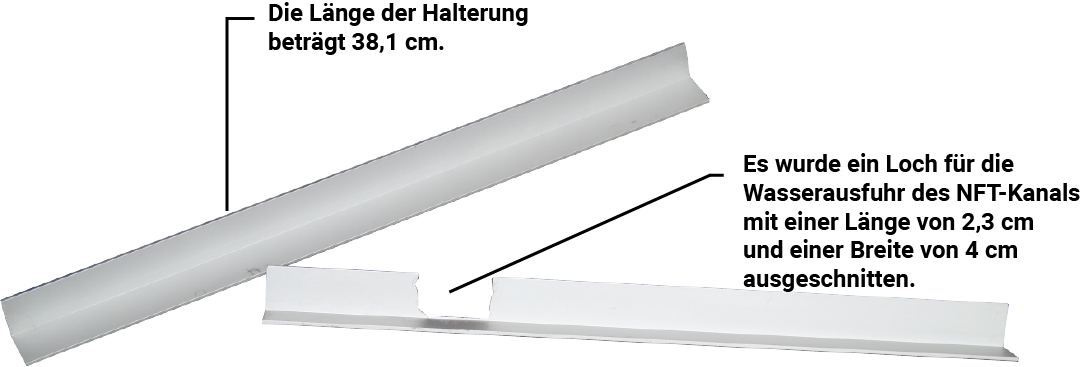
\includegraphics[width=0.5\textwidth]{images/NFT-Kanal_Halterung}
	    \caption{Halterung des \gls{NFT}-Kanals}
    \end{figure}
    \newpage
    \item [Anpassung des \gls{NFT}-Kanals]\mbox{} \\ 
    Die Pflanzennetze benötigten Löcher, in welchen sie in den \gls{NFT}-Kanal eingeschoben werden. Diese Löcher wurden laut der \gls{Sketchup}-Vorlage von Ponix Systems gebohrt und sind in einem Zickzackmuster angeordnet.\mbox{} \\
    \begin{figure}[ht]
        \centering
        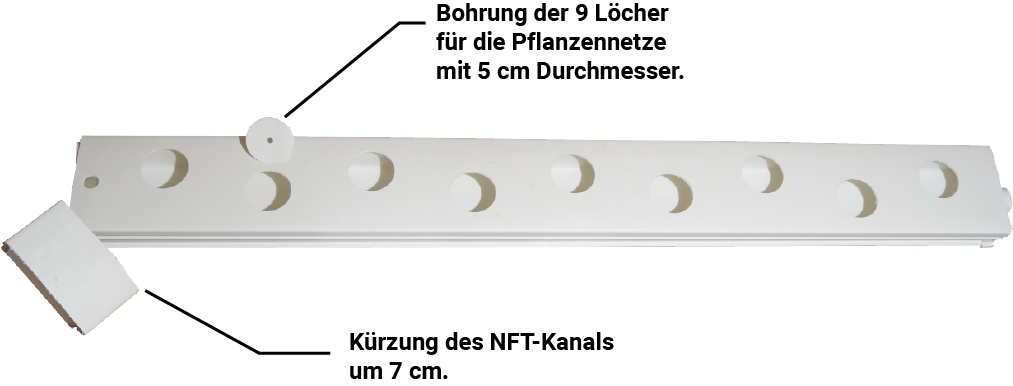
\includegraphics[width=0.5\textwidth]{images/NFT-Kanal_Mod}
	    \caption{Modifizierter \gls{NFT}-Kanal}
    \end{figure}\\
    Der zur Verfügung gestellte \gls{NFT}-Kanal war nicht an die Länge der Abdeckung/des Aquariums angepasst und musste in der Länge gekürzt werden.\\
    \item [Lochbohrungen der Abdeckungen]\mbox{} \\
    Damit die Pflanzen Platz haben um aus dem Aquarium auswachsen zu können mussten Löcher an genau der gleichen Position gebohrt werden wie im darunterliegenden \gls{NFT}-Kanal.\mbox{} \\
    \begin{figure}[ht]
        \centering
        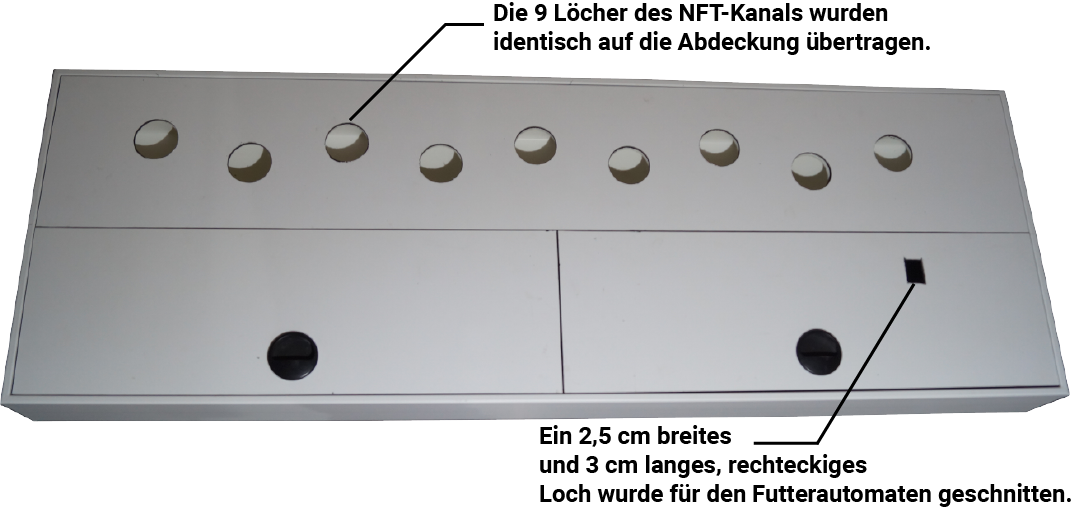
\includegraphics[width=0.5\textwidth]{images/Aufsatz_komplett_Mod}
	    \caption{Halterung des \gls{NFT}-Kanals}
    \end{figure}\\
    Der Futterautomat wurde auch durch ein Loch an der rechten unteren Abdeckung befestigt.
    \item [Herstellung einer Befestigung der LED-Halterung]\mbox{} \\
    Zu Anfang mussten die für die \gls{LED}-Halterung konzipierte Aluminium Bleche in der Breite und Länge zugeschnitten werden. Danach wurden die beiden Blechstreifen so gebogen, dass die im Vergleich zu dem Aquarium kürzere Halterung passend befestigt werden konnte.\mbox{} \\
    \begin{figure}[ht]
        \centering
        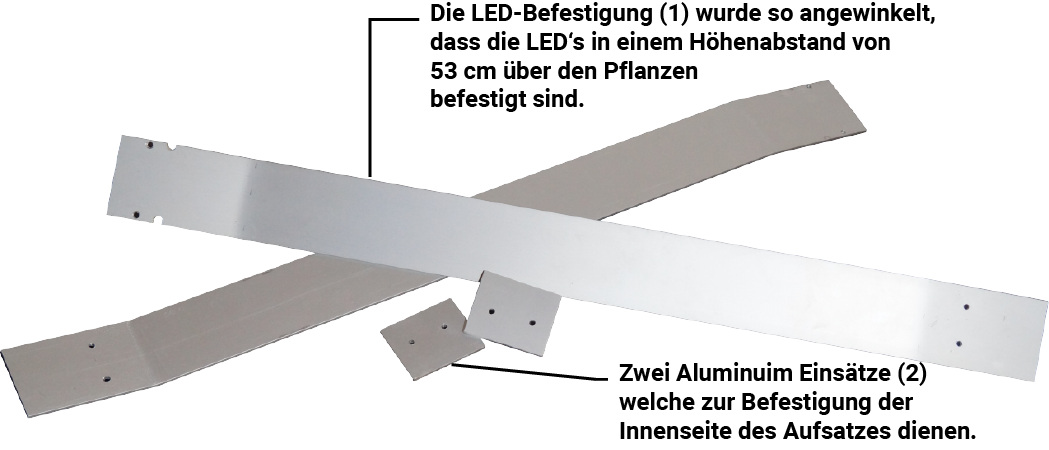
\includegraphics[width=0.5\textwidth]{images/LED_Befestigung}
	    \caption{Befestigungen der LED-Halterung}
    \end{figure}\\
    \mbox{} \\
    Um die Befestigung (gebogene Aluminium Blechstreifen) an der Halterung und an dem Aquariumaufsatz zu befestigen wurden Löcher in die Befestigung und den Aufsatz gebohrt. Ein stabiler Sitz der Befestigung an dem Aufsatz konnte ohne zusätzliche Aluminium Einsätze (in dem darüberstehenden Bild mit der Nummer 2 makiert) nicht erreicht werden, weil der Aufsatz nur aus Kunststoff besteht. Deswegen wurden kleine Aluminium Einsätze zurechtgeschnitten und die gleichen Bohrungen wie bei der Befestigung vorgenommen.\mbox\\
    \begin{figure}[ht]
        \centering
        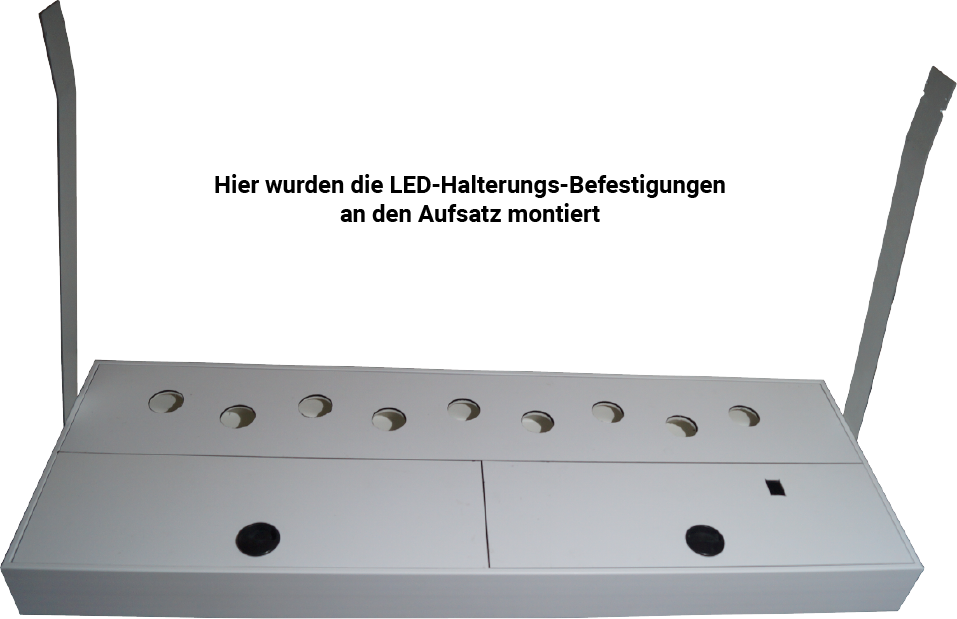
\includegraphics[width=0.5\textwidth]{images/Aufsatz_komplett_LED}
	    \caption{Aquariumaufsatz mit LED-Befestigung}
    \end{figure}\mbox{} \\
    Alle Teile wurden nun zusammengeschraubt. Das folgende Bild zeigt den vollständigen Prototypen. \mbox{} \\
    \begin{figure}[ht]
        \centering
        \includegraphics[width=1\textwidth]{images/Aufsatz_final}
	    \caption{Zusammengebauter Aquariumaufsatz}
    \end{figure}
\end{description}